\documentclass{article}
\usepackage[paper=portrait,pagesize]{typearea}
\usepackage{tikz}
\usepackage{caption}
\usepackage{subcaption}
\usepackage{fontawesome5}

\usepackage{amsmath}
\usepackage{pgfplots}
\pgfplotsset{compat=1.12}


\usetikzlibrary{backgrounds,automata}
\usetikzlibrary{positioning, shadows}
\usetikzlibrary{mindmap,backgrounds}
\usetikzlibrary{shapes.geometric}

\usepackage{geometry}
 \geometry{
 legalpaper,
 total={170mm,257mm},
 left=10mm,
 top=20mm,
 }


\begin{document}
\newpage
\KOMAoptions{paper=landscape,pagesize}

\begin{figure}
\begin{subfigure}[c]{.3\textwidth}
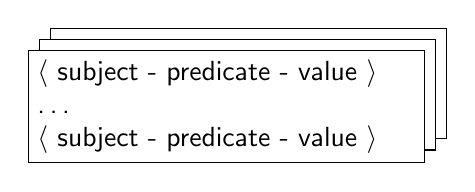
\begin{tikzpicture}[font=\sffamily]
\tikzstyle{doc}=[%
minimum height=4em,
minimum width=3em,
draw, fill=white
]
   \node[doc, text width=4.8cm] (doc) {$\langle$ subject - predicate - value $\rangle$};
   \node[doc, below left = 4pt and 4pt of doc.north east, text width=4.8cm] (doc2) {$\langle$ subject - predicate - value $\rangle$};
   \node[doc, below left = 4pt and 4pt of doc2.north east, text width=4.8cm] (doc) {$\langle$ subject - predicate - value $\rangle$ \\ \dots \\ $\langle$ subject - predicate - value $\rangle$ };
\end{tikzpicture}
\caption{}
\label{fig:read_nt_triles}
\end{subfigure}%
\begin{subfigure}[c]{.3\textwidth}
\[
D = \begin{bmatrix} 
    d_{11} & d_{12} & d_{13} & \dots \\
    \vdots & \ddots & \dots & \vdots\\
    \vdots & \ddots & \dots & \vdots\\
    d_{n1} & \dots  & \dots & d_{nn} 
    \end{bmatrix}
\]
\caption{}
\label{fig:distance_matrix}
\end{subfigure}%
\begin{subfigure}[c]{.45\textwidth}
\centering
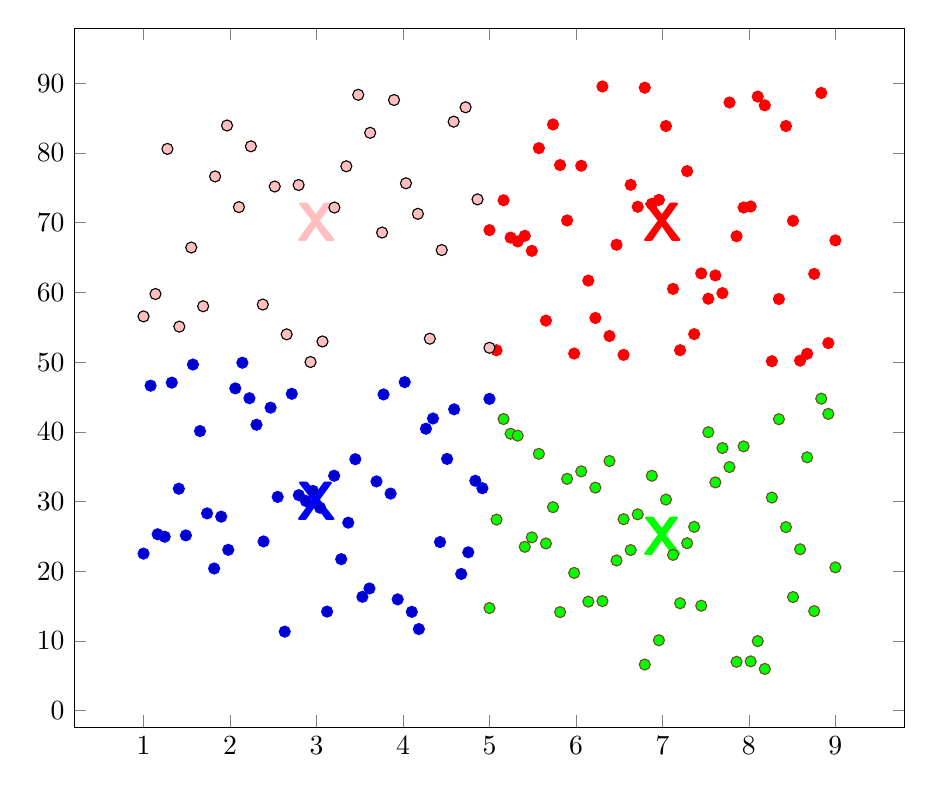
\begin{tikzpicture}
  \begin{axis}[width=\linewidth]
       % First cluster (blue)
       \node[text=blue,font=\sffamily\bfseries,scale=2] at (3,30) {X};
       \addplot+[y filter/.expression={y+10},only marks,mark=*,samples=50,domain=1:5] {40*rnd};

       % Second cluster (red)
       \node[text=red,font=\sffamily\bfseries,scale=2] at (7,70){X};
       \addplot+[y filter/.expression={y+50},only marks,mark=*,mark options={fill=red},samples=50,domain=5:9] {40*rnd};

       % Third cluster (green)
       \node[text=green,font=\sffamily\bfseries,scale=2] at (7, 25){X};
       \addplot+[y filter/.expression={y+5},only marks,mark=*,mark options={fill=green},samples=50,domain=5:9] {40*rnd};

       % Fourth cluster (pink)
       \node[text=pink,font=\sffamily\bfseries,scale=2] at (3,70){X};
       \addplot+[y filter/.expression={y+50},only marks,mark=*,mark options={fill=pink},samples=30,domain=1:5] {40*rnd};
       
  \end{axis}
\end{tikzpicture}
\caption{}
\label{fig:clustering}
\end{subfigure}%
\begin{subfigure}[c]{.5\textwidth}
\centering
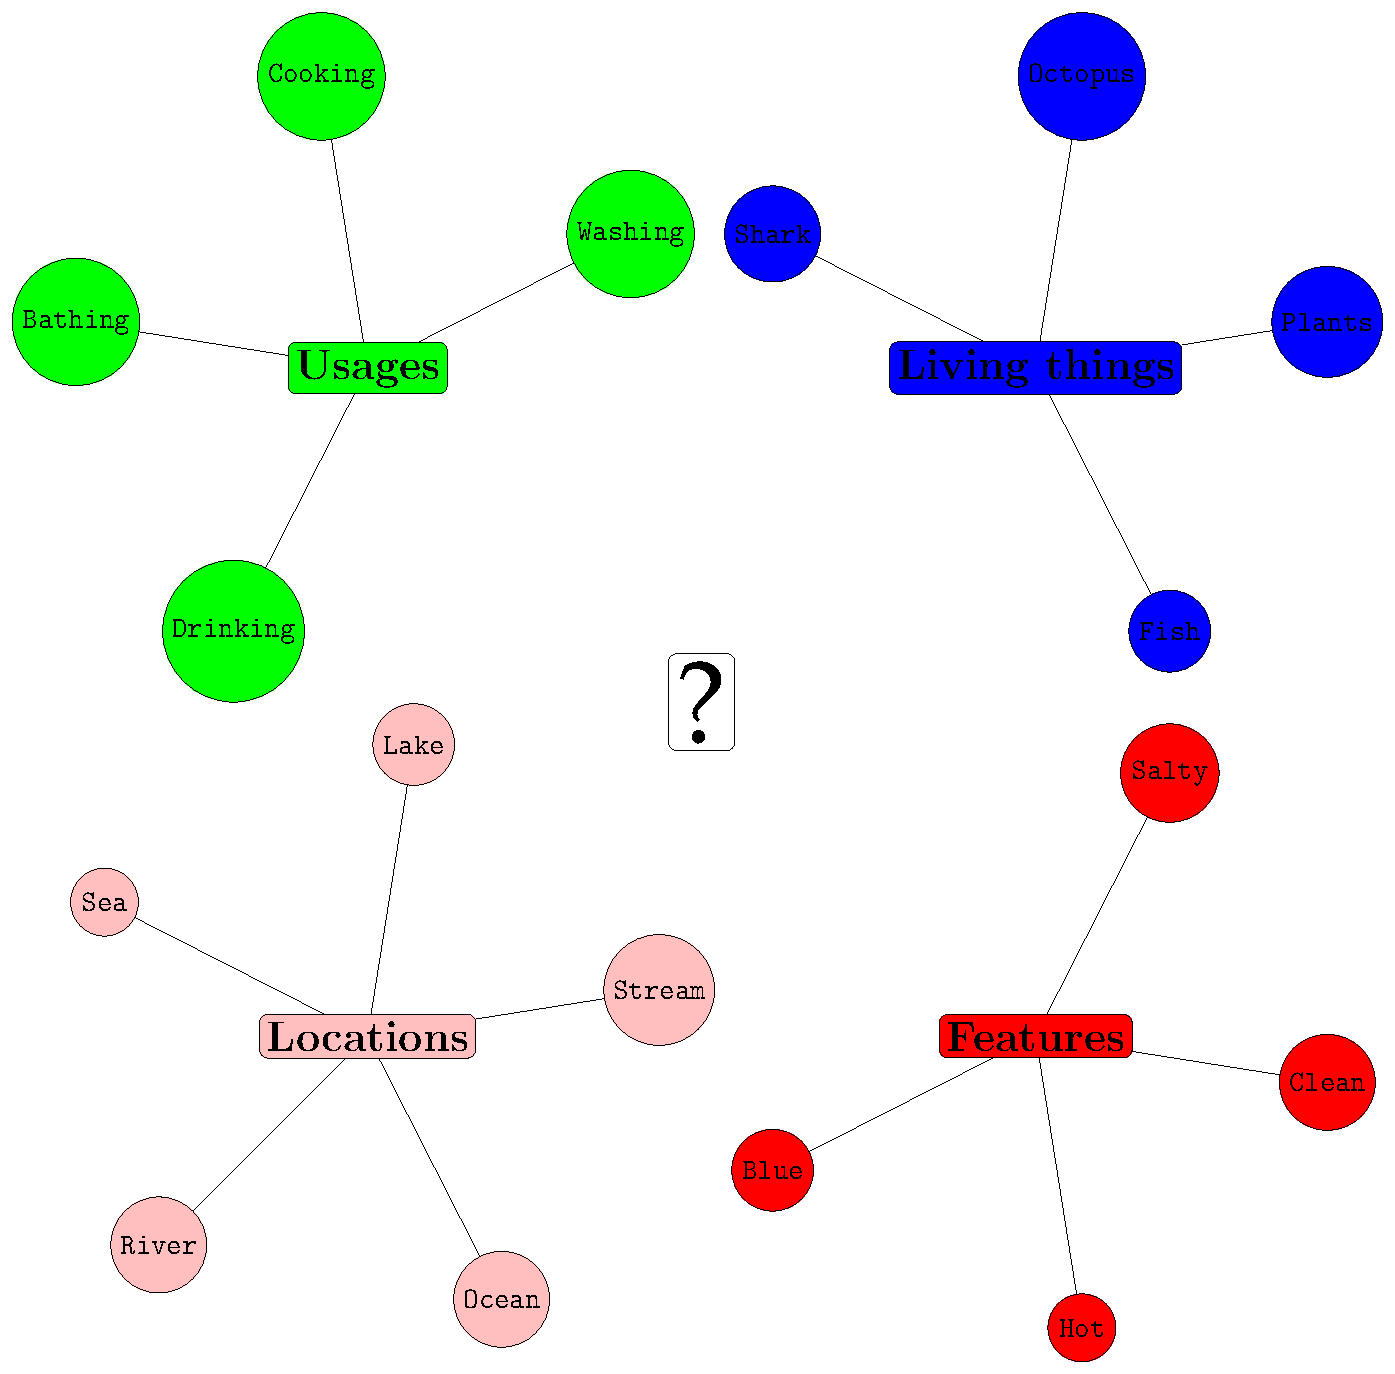
\includegraphics[scale=0.2]{img/Water_Semantic_Map_sans_main_term.pdf}
\caption{}
\label{fig:infer_alpha}
\end{subfigure}%
\begin{subfigure}[c]{.38\textwidth}
\centering
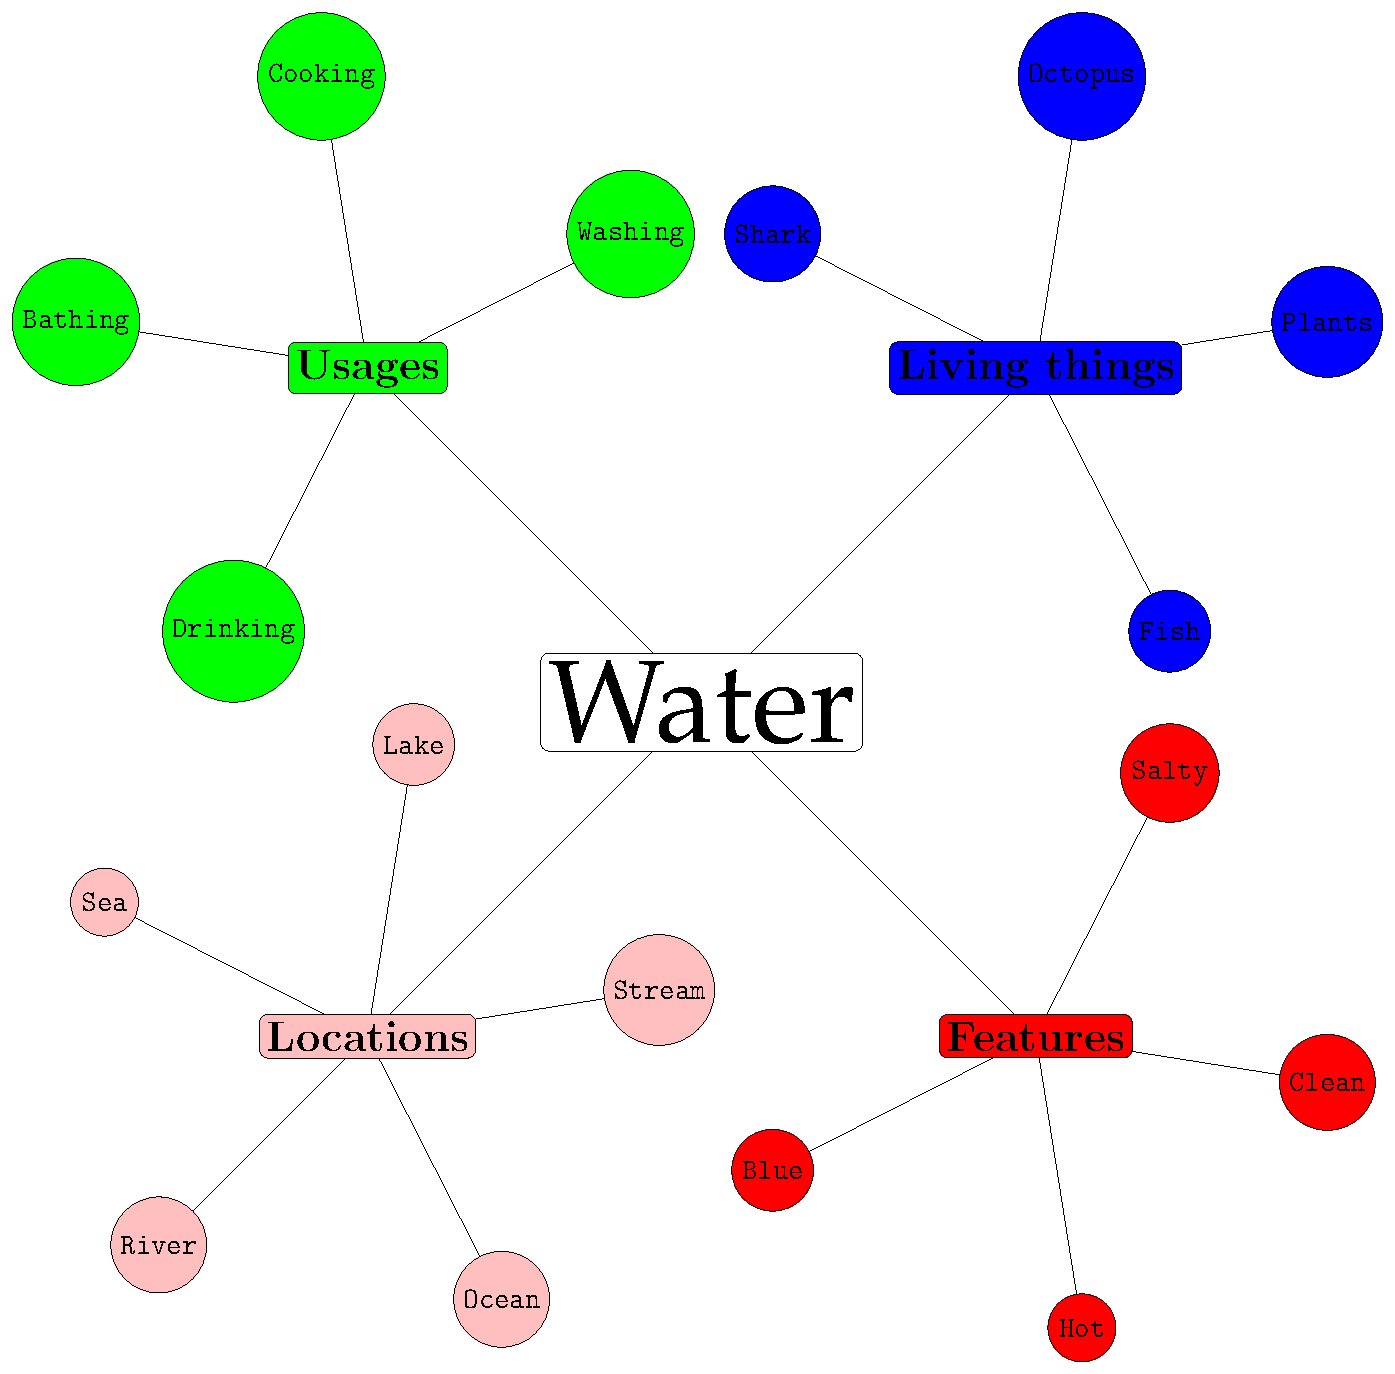
\includegraphics[scale=0.2]{img/Water_Sematic_Map_colour.pdf}
\caption{}
\label{fig:assemble_semantic_map}
\end{subfigure}
\caption{Semantic mapping process}
\end{figure}


\end{document}